

\chapter{Softwarearchitektur der bestehenden Software}

    Analysemethoden der Informatik für Software sind in der Regel für die verschiedenen Design-Phasen einer Software entwickelt worden.
    Eine von mir durchgeführte Recherche ergab,dass sich Analyse-Tools und Methoden für bestehende Software vor
    Allem darauf fokussieren die Performance, Speichermanagement und Benutzererfahrung zu bewerten.
    Die Architektur einer Software spielt dabei eine untergeordnete Rolle.
    Für die Neuentwicklung der bestehenden Software wird im Folgenden die Programmstruktur dargestellt und analysiert,
    sodass eine Bewertung der Programmkomponenten erfolgen kann.
    \\
    In einem C\# - Projekt sind UI und Logik in getrennten Dateien implementiert. XAML- Dateien sind eine angepasste
    Form von XML-Dateien und legen somit fest wie das GUI gerendert wird.
    XAML.CS Dateien enthalten die dahinterliegende Logik inklusive Schnittstellen zu anderen Programmteilen.
    Am Beispiel des Startbildschirm des Programms \"Lagerverwaltung 3.0\" wird der grundlegende Programmaufbau geschildert.
    Im Weiteren wird wegen der Komplexizität und des fehlenden Mehrwerts darauf verzichtet.
    Ich verzichte aus den gleichen Gründen auf die detaillerte Funktionsweise der graphischen ELemente und der Events
    sowie ihrer Eventhandler.
    \\
    In den erstellen Klassendiagrammen ist jedoch gut ersichtlich welche Klasse Events nutzt. Die Klasse
    \verb|INotifyPropertyChanged| stellt die benötigten Listeners dafür bereit und wird an andere Klassen vererbt.

    \subsection {Lagerverwaltung 3.0}

    Wie in dem einleitenden Abschnitt angekündigt wird zunächst der grundlegende Aufbau des Programms aufgelistet.
    \\
    Die Datei \verb|App.xaml| ist der Einstiegspunkt des Programms.
    In ihr wird ein Objekt der Application-Klasse mit allen benötigten Ressourcen erzeugt.
    Als Start URL ist \verb|MainWindow.xaml| angeben.
    \\
    In der Datei ist beschrieben wie der Startbildschirm gerendert wird.
    Zunächst wird ein Banner gerendert, bestehend aus dem Titel des Programms, dem Logo des Instituts und der $\mu$Plant
    (Siehe Abb. 2.1 Bereich \"A\").
    Es werden außerdem alle benötigten Daten-Objekte erzeugt.
    Sie lassen sich wie folgt einteilen:
    \\
    \begin{itemize}
        \item Objekte und Variablen, die dem Lager zugeordnet sind:
            \begin{itemize}
                \item Ein Objekt \verb|inventory| der Klasse \verb|Inventory| für das Inventar mit \verb|null| initialisiert.
                \item Ein Objekt \verb|storageMatrix| von der Klasse \verb|PalletMatrix| erzeugt.
                \item Ein Object \verb|commissionMatrix| von der Klasse \verb|PalletMatrix| erzeugt.
                \item Ein Objekt \verb|mobileRobot| von der Klasse \verb |MobileRobot| erzeugt.
                \item Außerdem eine Variable \verb|lastCupRead| vom Datentyp \verb|ushort| (16-Bit-Ganzzahl, vorzeichenlos) mit 0 initialisiert.
            \end{itemize}
            \item Objekte und Variablen initialisiert, die dem ABB Controller zugeordnet sind:
            \begin{itemize}
                \item Ein Objekt \verb|commands| von der Klasse \verb|controllerCommandList|.
                \item Ein Objekt \verb|controllerProperties| von der Klasse \verb|RobotControllerProperties|.
                \item Ein Objekt \verb|controllerBase| von der Klasse \verb|RobotControllerBas|, mit dem Initialisierungswert \verb|null|.
                \item Ein Objekt \verb|controllerSim| von der Klasse \verb|RobotSimulator|.
            \end{itemize}
    \end{itemize}
    Im Constructor der Klasse \verb|MainWindow| werden außerdem der ModBus und der Roboter Controller initialisiert
    und wie in Abb. 2.1 gerendert (Bereiche gekennzeichnet durch die Buchstaben \"B\" und \"C\").
    Die Produktliste wird aus der Datei \verb|Produkte.db| geladen und gerendert (Abb. 2.1 Bereich \"D\").
    Daten des Lagers und des mobilen Roboters sowie die Kommissionsdaten werden aus der Datei \verb|CommissionData.db|
    geladen und anschließend das Inventar gerendert:
    Es wird einerseits eine Produktliste im Bereich \"E\" in Abb. 2.1 erzeugt, die um die gelagerte Menge ergänzt ist.
    Produkte ohne Lagermenge können mit einer Checkbox wahlweise ein- und Ausgeblendet werden.
    Andererseits werden die Daten genutzt um im Bereich \"G\" der Abbildung das Lager zu visualisieren.
    Die drei Reihen \"TOP\", \"MIDDLE\" und \"BOTTOM\" solen die drei Regalböden des Lagerregals nachbilden.
    Die Slkots A1\ldots A6, H1\ldots H6 sowie  H7\ldots H12 sind die Plätze für je eine Palette, die wiederum Platz für
    je zwei Becher hat.
    Der Ursprung dieser Bezeichnung konnte während der Vorbereitungen auf diese Arbeit nicht geklärt werden.
    Das reale Pendant ist mit L1\ldots L18 gekennzeichnet.
    \\
    Im Bereich \"F\" werden alle Ereignisse der Software als text angezeigt.
    Das können Fehler sein aber auch Fortschritte im Programmablauf.
    \\
    Im Mittleren Bereich ist die Anordnung von Roboter, Andockstation und Kommissioniertisch symbolisiert.
    Der \"Start\"-Knopf startet den Automatikbetrieb. Wenn keine Verbindung zum Mosbus hergestellt werden kann,
    wird dem Benutzer angeboten die Vorgänge zu simulieren. Im Klassendiagramm Abb. 2.2 wird jedoch schnell deutlich,
    dass dieser Simulationsbetrieb nicht dazu genutzt werden kann um etwaige Fehler zu erkennen, da dazu eine ganz
    andere Klasse verwendet wird.
    Im Bereich \"Mobile Robot\" wird nach erfolgreichem Andocken das erkannte Produkt angezeigt.
    Dem Bediener wird hier angeboten die Daten manuell zu manipulieren oder Details auszublenden.
    Im Bereich \"Workbench\" werden bis zu zwei Paletten mit ihrem Inhalt gerendert.
    Auch hier wird dem Benutzer angeboten die Daten per Hand zu manipulieren.

    \begin{figure}[ht]
        \label{fig:figure}
        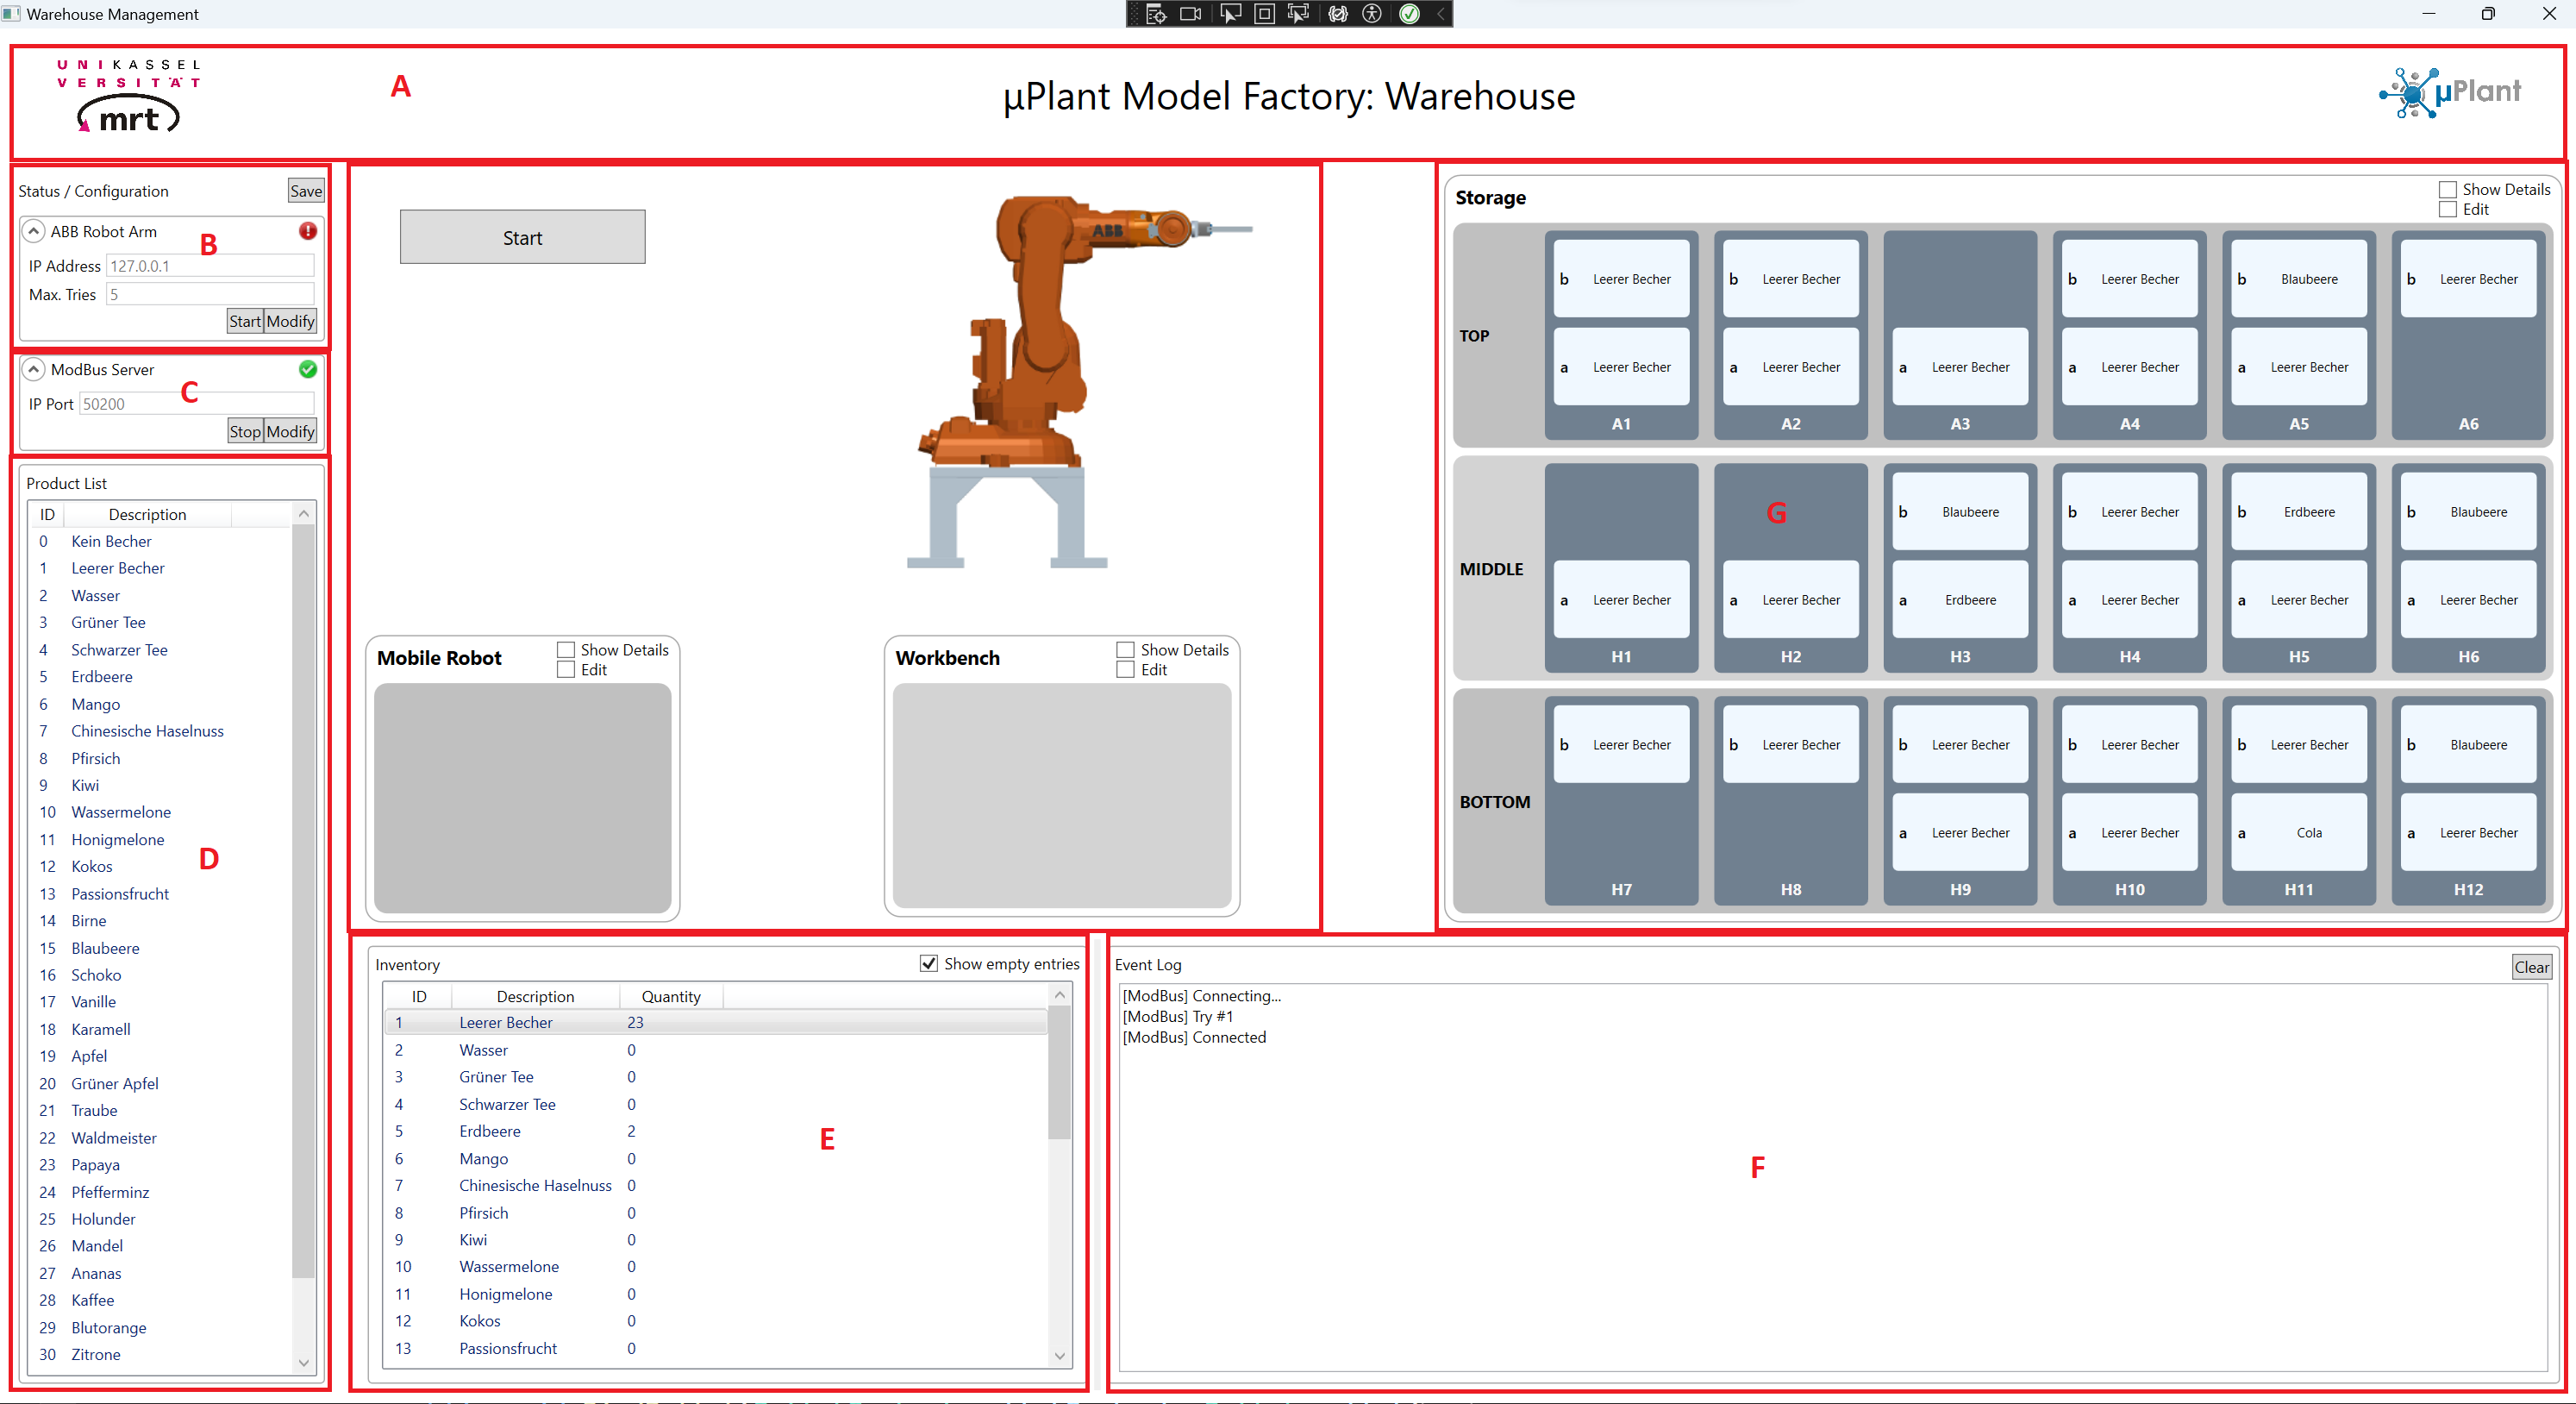
\includegraphics[width = \textwidth ]{Bilder/LV_Startbildschirm}
        \caption[Ansicht des Startbildschirms]
        {\small Startbildschirm der Anwendung, zur besseren Beschreibung sind die Bedienbereiche rot umrandet und mit
        Buchstanben gekennzeichnet}
        \centering
    \end{figure}

    \subsubsection{Datenstruktur}

    Die bestehende Software dient dazu Lagerpakete vom mobilen Roboter auf die Werkbank oder ins Lager zu bewegen.
    Oder alle möglichen Kombinationen davon.
    Das Konzept der $\mu$Plant beschränkt sich dabei auf eine Palette, die so ausgeführt ist, dass der Greifer des
    Industrieroboters sie sicher bewegen kann.
    Im Wesentlichen ist es ein Quader mit zwei seitlichen Längsnuten.
    Eine Palette enthält zwei senkrechte Bohrungen, die es ermöglichen je einen Becher aufzunehmen.
    Ein Becher ist ein transparentes, zylindrisches Gefäß aus Acrylglas mit einem Absatz, der etwa mittig in der
    Höhe angebracht ist, sodass der Greifer die Becher einzeln bewegen kann.
    Es wird also immer entweder
    \begin{itemize}
        \item Eine Palette
        \item Ein Becher
        \item eine Palette mit einem oder mehreren Bechern
    \end{itemize}
    bewegt.
    Der Programmierer hat sich diese Struktur angeeignet und in der Datenmodellierung umgesetzt.
    In Abb. 2.2 ist gut ersichtlich, dass die Klasse \verb|StorageElementBase| an die Klassen \verb|Cup| und \verb|Pallet|
    vererbt (schmale Linie mit leerem Pfeil, in Anlehnung an UML). Eigenschaften, die sowohl Palette als auch den
    Becher betreffen sind in dieser Klasse implementiert.
    Weiterhin findet sich das Lager als eigene Klasse \verb|Inventory| und der mobile Roboter als \verb|MobileRobot| wieder.
    Die \verb|Inventory|-Klasse ist jedoch nicht das Lager im Sinne von Abb 2.1 Bereich \"G\", sondern auf die Liste in
    Bereich \"E\".
    Ansonsten versucht das Datenmodell nicht weiter reale Prozesse im Programm abzubilden.
    \\
    \begin{figure}[ht]
        \label{fig:figure2}
        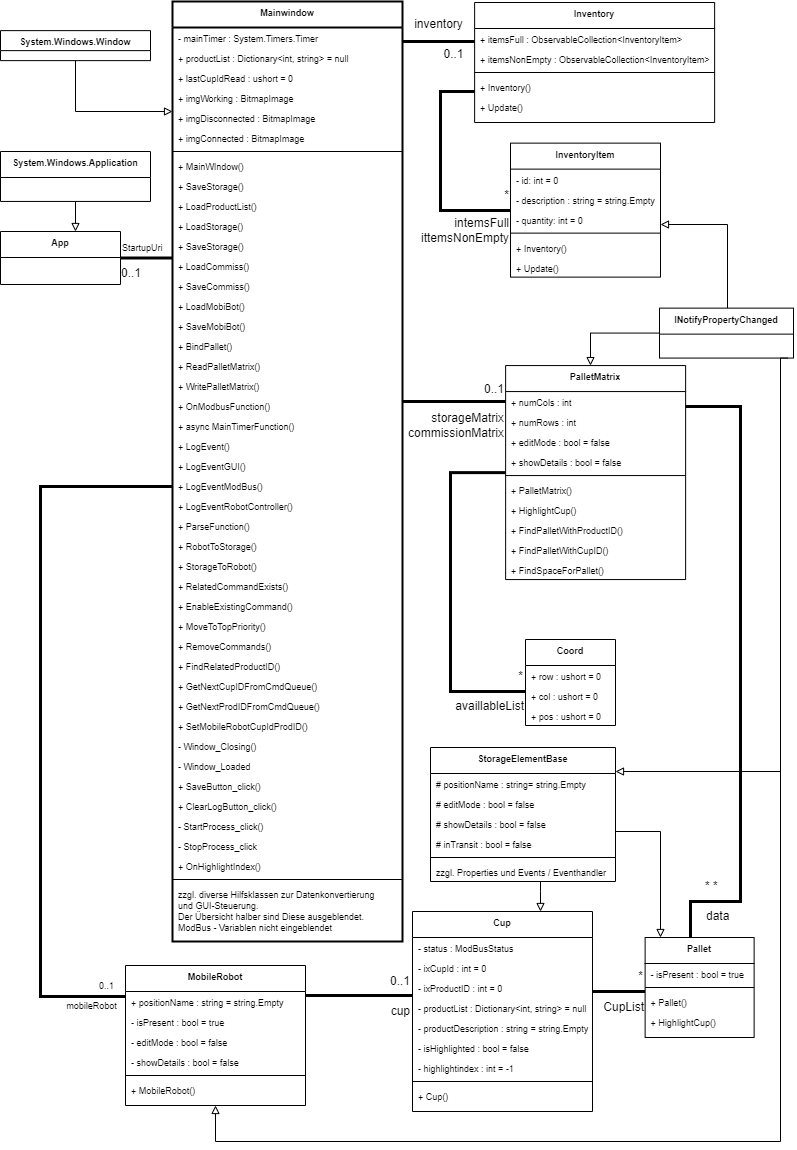
\includegraphics[width = \textwidth ]{Bilder/LV_Klassendiagramm_Datenmodell}
        \caption[Klassendiagramm Datenmodells ]
        {\small Klassendiagramm der MainWindow-Klasse mit vererbenden- und Datenmodell - Klassen }
        \centering
    \end{figure}

    Zentrales Element ist die \verb|MainWindow| Klasse.
    Sie implementiert eigentlich eine Interface-Klasse \verb|System.Windows.Window| und ist somit als GUI-Element gedacht.
    Der Programmierer hat sie allerdings als Daten-Hub verwendet.
    Wie oben geschildert werden beim Rendern des Fensters alle benötigten Datenobjekte erzeugt oder aus Dateien geladen.
    \begin{itemize}
        \item In der Klasse \verb|Inventory| wird der Inhalt der Datei \verb|Produkte.db| in zwei Listen geladen, sodass
        eine Liste mit lagernden Produkten und eine vollständige Produktliste gespeichert werden.
        Eine Instanz \verb|inventory| wird zur Laufzeit erzeugt. Wenn die Dateien \verb|Produkte.db| und
        \verb|StorageData.db|zu dem Zeitpunkt nicht verfügbar ist, stürzt das Programm ab.
        \item In der Klasse \verb|PalletMatrix| wird die Datei \verb|StorageData.db| bzw. \verb|CommissionData.db|
        geladen um einen zweidimensionalen Array \verb|data| zu erzeugen.
        Jedes Array-Element ist ein Objekt der Klasse \verb|Pallet| und Enthält eine Liste \verb|CupList| von Objekten
        der Klasse \verb|Cup|.
        Diese Struktur wird dazu verwendet um das reale Lager nachzubilden.
        Zur Laufzeit werden zwei Objekte der Klasse \verb|PalletMatrix| erzeugt:
        \item \item \verb|storageMatrix| bildet das Datenmodell um die Visualisierung in Abb. 2.1 Bereich \"G\" zu realisieren.
        \item \item \verb|commissionMatrix| bildet das DatenModell für die Visualisierung des mobilen Roboters und der
        Workbench. 
    \end{itemize}
    \begin{figure}[ht]
        \label{fig:figure3}
        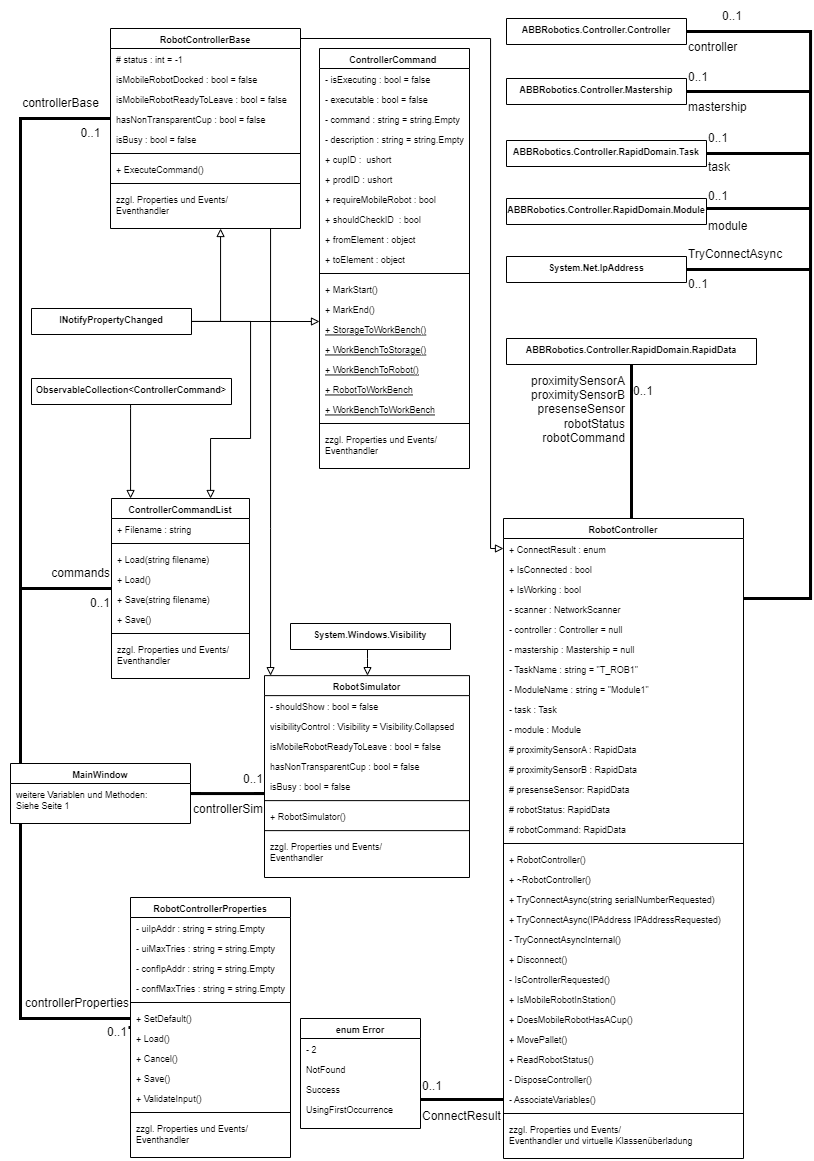
\includegraphics[width = \textwidth ]{Bilder/LV_Klassendiagramm_ABBController}
        \caption[Klassendiagramm ABB Controller ]
        {\small Klassendiagramm der MainWindow-Klasse mit Klassen aus dem ABB Controllerframework. }
        \centering
    \end{figure}

    \begin{figure}[ht]
        \label{fig:figure4}
        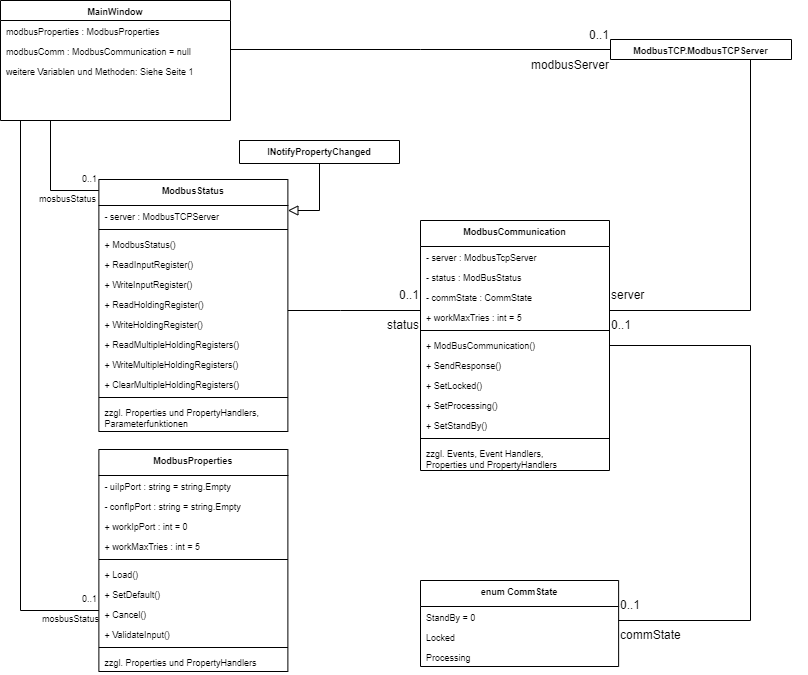
\includegraphics[width = \textwidth ]{Bilder/LV_Klassendiagramm_Modbus}
        \caption[Klassendiagramm Modbus ]
        {\small Klassendiagramm der MainWindow-Klasse mit Mosbus-Klassen }
        \centering
    \end{figure}

    \begin{figure}[ht]
        \label{fig:figure5}
        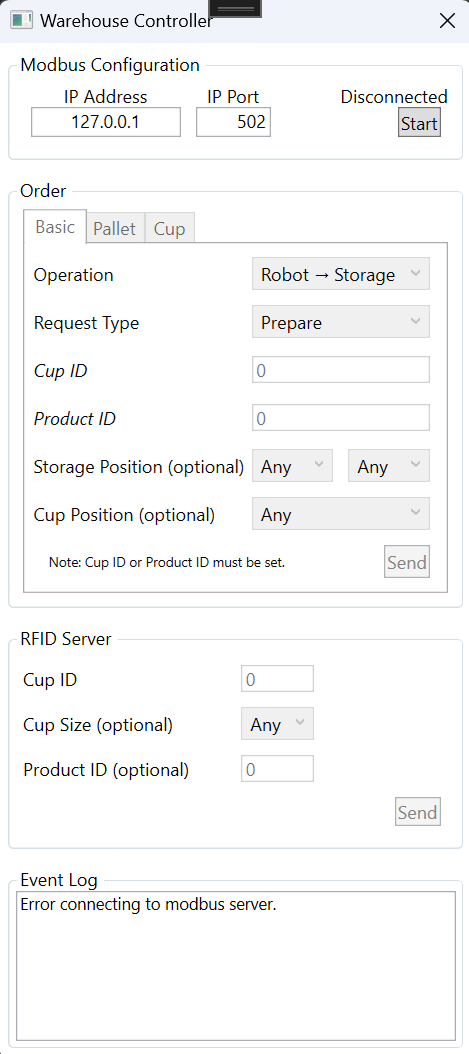
\includegraphics[height = \textheight ]{Bilder/Controller_Startbildschirm}
        \caption[Ansicht des Controller- Startbildschirm ]
        {\small Ansicht des Controller Startbildschirms. }
        \centering
    \end{figure}

    \begin{figure}[ht]
        \label{fig:figure6}
        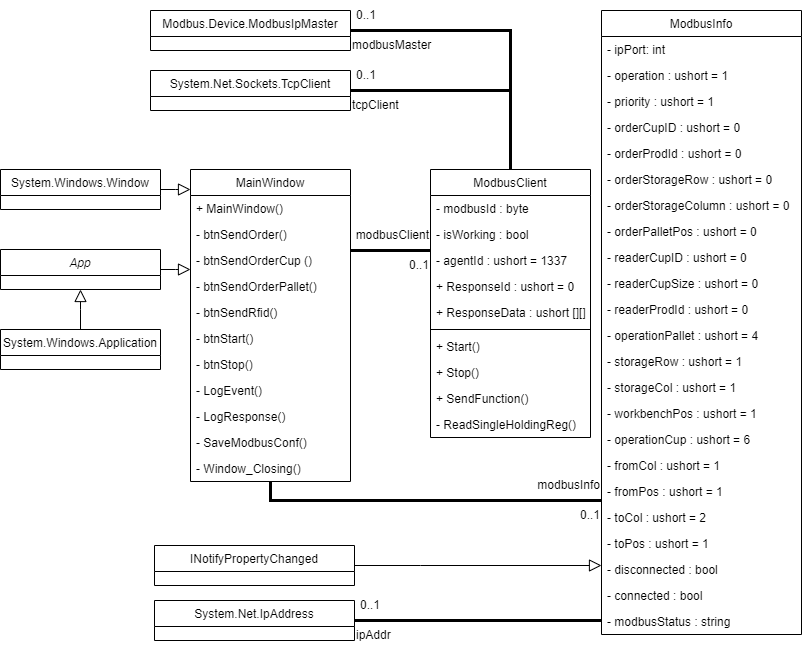
\includegraphics[width = \textwidth ]{Bilder/C_Klassendiagramm}
        \caption[Klassendiagramm des Controllers ]
        {\small Klassendiagramm des Warehouse-Controllers mit allen vererbenden Klassen jedoch ohne Klassen die
        lediglich Datentypen konvertieren.}
        \centering
    \end{figure}

    \begin{figure}[ht]
        \label{fig:figure7}
        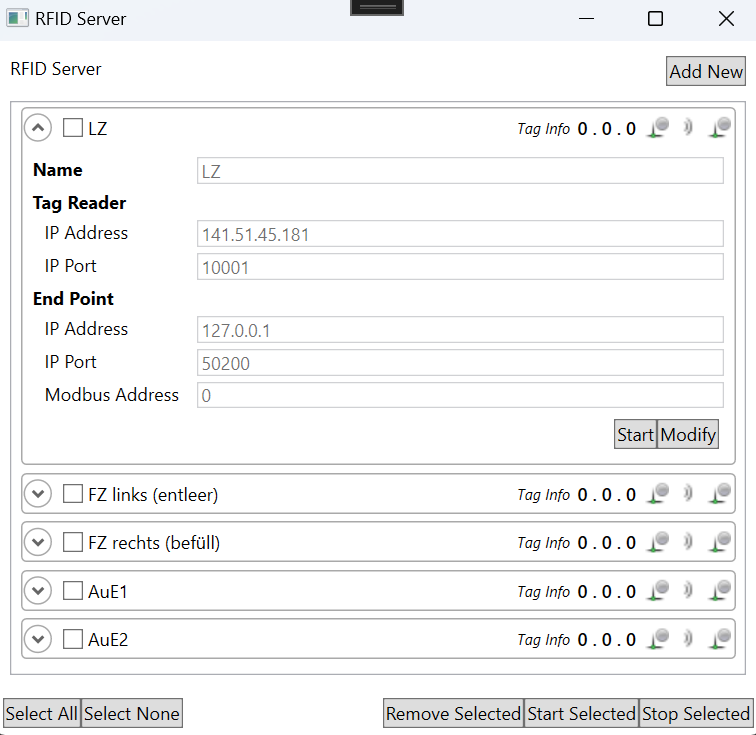
\includegraphics[height = \textwidth ]{Bilder/RFIDServer_Bildschirm}
        \caption[Startbildschirm des Programms RFID-Server]
        {\small Startbildschirm des Programms RFID-Server}
        \centering
    \end{figure}

    \begin{figure}[ht]
        \label{fig:figure8}
        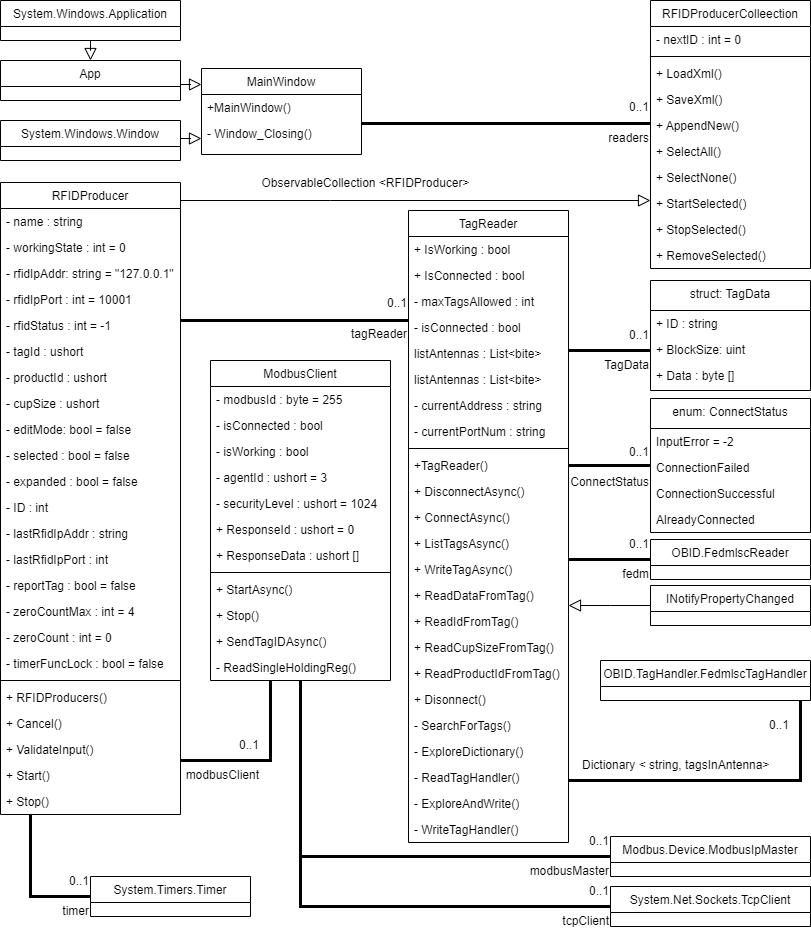
\includegraphics[width = \textwidth ]{Bilder/RFID_Klassendiagramm}
        \caption[Klassendiagramm des Programms RFID-Server ]
        {\small Klassendiagramm des Programms RFID-Server mit allen vererbenden Klassen jedoch ohne solche die
        lediglich Typen konvertieren.}
        \centering
    \end{figure}


    \begin{itemize}
        \item Der rote , mit "1" markierte Bereich im Startbildschirm dient dazu die Verbindungsdaten zum ModBus zu konfigurieren. Über entsprechende Taste kann die Eingabe der beiden Felder aktiviert/deaktiviert werden. Über die Start-Taste wird die VErbindung hergestellt.
        An der Stelle des sichtbaren roten Ausrufezeichen-Symbol wird ein grüner Haken sichtbar, wenn die Verbindung korrekt hergestellt wurde.
        \item Der blaue, mit "2" markierte Bereich dient dazu gesondert den ModBus-Port einzustellen.
        \item Der grüne, mit "3" markierte Bereich ist eine Listenansicht, in der jedes mögliche Produkt mit seiner zugeordneten ID abgebildet ist.
        Die Liste ermöglicht dem Benutzer einen schnellen Überblick über mögliche Produkte.
        \item Der gelbe, mit "4" markierte Bereich ist die Übersicht über das aktuelle Geschehen. Im linken, unteren Bereich ist der Lagerplatz des mobilen Roboters symbolisiert.
        Im rechten, unteren Bereich ist der Lagerplatz der Werkbank symbolisiert. Beide Symboliken verfügen über je einen Lagerplatz, wobei die real doppelte Ausführung der Werkbank nicht umgesetzt wurde.
        \item die violetten Bereiche "5" und "6" bilden die Visualisierung des Lagers. In Bereich 6 sind die 18 Lagerslots so dargestellt wie das reale Regal aufgebaut ist. Einzig die Lagerort-Bezeichnung ist anders.
        Im Bereich "5" werden alle möglichen Produkte in einer Liste mit der gelagerten Menge angezeigt. Wahlweise können alle Produkte ausgeblendet werden, die keine Bestand haben.
        Mit Klick auf ein Produkt, egal ob im Bereich "5" oder "6", werden alle passenden Einträge farblich hervorgehoben, sodass auf einen Blick erkennbar ist, wo die Lagermenge im Lager wirklich abgebildet ist.
        \item Im grünen, mit "7" gekennzeichneten Bereich ist ein Eventlogger implementiert. Wann immer ein für den Benutzer relevantes Ereignis eintritt, wird hier eine entsprechende Meldung angezeigt.
    \end{itemize}


    \subsection {RFID Server}

    \subsection {Controller}

